\documentclass[12pt]{article}

%Packages add more power to LaTeX documents
\usepackage{fullpage} %Otherwise there will be a lot of wasted space at the margins
\usepackage{enumerate} %For the multi-part problem in example #4
\usepackage{amsthm} %For proof environment
\usepackage{amsmath} %For math symbols (like the black square)
\usepackage{graphicx,float,wrapfig} %Including graphics like PDFs and some image formats.


\author{Annabelle Cormia}
\title{CSCI 430: Homework 2}
\newcommand\tab[1][1cm]{\hspace*{#1}}

\begin{document}
\maketitle

Tyler Archer and I collaborated on this assignment.\newline

\section{Chapter 2.1 (2.1-1 through 2.1-4)}

%Number \item tags
\begin{enumerate}
 
  \item See Figure \ref{figure1}.

	\begin{figure}[h!]
	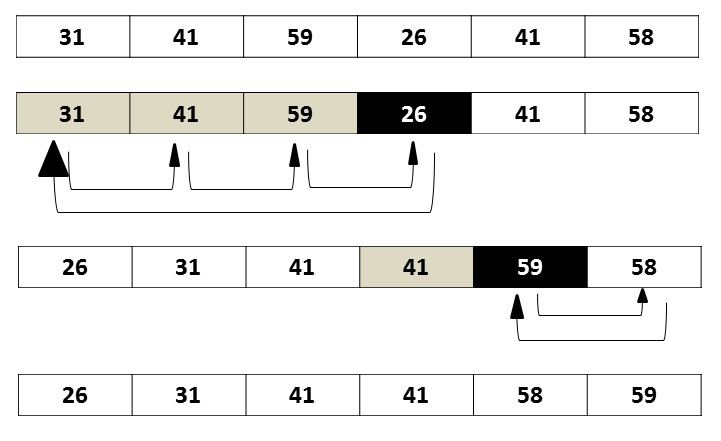
\includegraphics[width=7cm]{Graph3.jpg}
	\caption{Illustration of the operation of INSERTION-SORT on the array A = (31, 41, 59, 26, 41, 58).}
	\label{figure1}
	\end{figure}

  \item INSERTION-SORT (A) \\
	1 \tab	for j = 2 to A.length \\
	2 \tab \tab	key = A[j] \\
	3 \tab \tab	// Insert A[j]  into the sorted sequence A[1.. j - 1]. \\
	4 \tab \tab	 i = j - 1 \\
	5 \tab \tab	while i $>$ 0 and A[i] $>$ key \\
	6 \tab \tab \tab	 A[i + 1] = A[i] \\
	7 \tab \tab \tab	 i = i - 1 \\
	8 \tab \tab	A[i + 1] = key \\

  \item LINEAR-SEARCH (A) \\
	1 \tab for i = 1 to A.length \\
	2 \tab \tab while v $\neq$ A[i] \\
	3 \tab \tab \tab i = i + 1 \\
	4 \tab \tab if v = A[i] \\
	5 \tab \tab \tab return i \\
	6 \tab if i $>$ A.length \\
	7 \tab \tab return NIL \\

	Initialization: We start by showing that the loop invariant holds before the first loop iteration, when i $=$ 1. The loop invariant is vacuously true because it is empty. \\

	Maintenance: Next, we must show that each iteratino maintains the loop invariant. The while loop works by moving through A until it finds a value whose index equals v. Each time it does not find a value whose index matches v, it increments i to keep checking. If v equals A[i], then i is returned. If i exceeds the length of A, then NIL is returned. \\

	Termination: Finally, we examine what happens when the loop terminates. The condition causing the for loop to terminate is that i $>$  A.length which results in NIL. However, if a value i is found that equals v, that value is returned. Therefore, we conclude that the output is either an index i such that v $=$ A[i] or the value NIL if v does not appear in A. Thus the algorithm is correct.\\

  \item Adding two binary integers each of length n will result in an (n+1)-element array C. Suppose the two integers are stacked on top of each other so that the right-most element of each array is lined up. The carry digit will begin at 0. A, B, and carry are added together to produce sum for each column of digits. If sum is 0, then the carry element for the next column to be summed is 0 and the digit going into the array C is also 0. Array C holds the final sum of arrays A and B, and it has length n+1 to account for a surplus carry at the end of the addition. If the sum is 1, then the carry element is 0 and the next digit in the C array is 1. If the sum is 2, then the carry is 0 and the next digit in C is 1. If the sum is 3, then both the carry and next element in C are 1. Variable i is then decremented until the end of the array when the final carry is placed into the remaining spot in the C array.

	ADDING-BINARY-INTEGERS (A $+$ B)\\
	1   \tab carry = 0 \\
	2   \tab for n to i=1 // n is length of both A and B \\
	3   \tab \tab sum = A[i] + B[i] + carry \\
	4   \tab \tab if sum = 0 \\
	5   \tab \tab\tab carry = 0 \\
	6   \tab \tab \tab C[i + 1] = 0 \\
	7   \tab \tab if sum = 1 \\
	8   \tab \tab \tab carry = 0 \\
	9   \tab \tab \tab C[i +1]= 1 \\
	10 \tab \tab if sum = 2 \\
	11 \tab \tab \tab carry = 0 \\
	12 \tab \tab \tab C[i + 1] = 1 \\
	13 \tab \tab if sum = 3 \\
	14 \tab \tab \tab carry = 1 \\
	15 \tab \tab \tab C[i + 1] = 1 \\
	16 \tab \tab i$--$ \\
	17 \tab C[1] = carry \\
	
    
\end{enumerate}
    
\end{document}